\documentclass[1p]{elsarticle_modified}
%\bibliographystyle{elsarticle-num}

%\usepackage[colorlinks]{hyperref}
%\usepackage{abbrmath_seonhwa} %\Abb, \Ascr, \Acal ,\Abf, \Afrak
\usepackage{amsfonts}
\usepackage{amssymb}
\usepackage{amsmath}
\usepackage{amsthm}
\usepackage{scalefnt}
\usepackage{amsbsy}
\usepackage{kotex}
\usepackage{caption}
\usepackage{subfig}
\usepackage{color}
\usepackage{graphicx}
\usepackage{xcolor} %% white, black, red, green, blue, cyan, magenta, yellow
\usepackage{float}
\usepackage{setspace}
\usepackage{hyperref}

\usepackage{tikz}
\usetikzlibrary{arrows}

\usepackage{multirow}
\usepackage{array} % fixed length table
\usepackage{hhline}

%%%%%%%%%%%%%%%%%%%%%
\makeatletter
\renewcommand*\env@matrix[1][\arraystretch]{%
	\edef\arraystretch{#1}%
	\hskip -\arraycolsep
	\let\@ifnextchar\new@ifnextchar
	\array{*\c@MaxMatrixCols c}}
\makeatother %https://tex.stackexchange.com/questions/14071/how-can-i-increase-the-line-spacing-in-a-matrix
%%%%%%%%%%%%%%%

\usepackage[normalem]{ulem}

\newcommand{\msout}[1]{\ifmmode\text{\sout{\ensuremath{#1}}}\else\sout{#1}\fi}
%SOURCE: \msout is \stkout macro in https://tex.stackexchange.com/questions/20609/strikeout-in-math-mode

\newcommand{\cancel}[1]{
	\ifmmode
	{\color{red}\msout{#1}}
	\else
	{\color{red}\sout{#1}}
	\fi
}

\newcommand{\add}[1]{
	{\color{blue}\uwave{#1}}
}

\newcommand{\replace}[2]{
	\ifmmode
	{\color{red}\msout{#1}}{\color{blue}\uwave{#2}}
	\else
	{\color{red}\sout{#1}}{\color{blue}\uwave{#2}}
	\fi
}

\newcommand{\Sol}{\mathcal{S}} %segment
\newcommand{\D}{D} %diagram
\newcommand{\A}{\mathcal{A}} %arc


%%%%%%%%%%%%%%%%%%%%%%%%%%%%%5 test

\def\sl{\operatorname{\textup{SL}}(2,\Cbb)}
\def\psl{\operatorname{\textup{PSL}}(2,\Cbb)}
\def\quan{\mkern 1mu \triangleright \mkern 1mu}

\theoremstyle{definition}
\newtheorem{thm}{Theorem}[section]
\newtheorem{prop}[thm]{Proposition}
\newtheorem{lem}[thm]{Lemma}
\newtheorem{ques}[thm]{Question}
\newtheorem{cor}[thm]{Corollary}
\newtheorem{defn}[thm]{Definition}
\newtheorem{exam}[thm]{Example}
\newtheorem{rmk}[thm]{Remark}
\newtheorem{alg}[thm]{Algorithm}

\newcommand{\I}{\sqrt{-1}}
\begin{document}

%\begin{frontmatter}
%
%\title{Boundary parabolic representations of knots up to 8 crossings}
%
%%% Group authors per affiliation:
%\author{Yunhi Cho} 
%\address{Department of Mathematics, University of Seoul, Seoul, Korea}
%\ead{yhcho@uos.ac.kr}
%
%
%\author{Seonhwa Kim} %\fnref{s_kim}}
%\address{Center for Geometry and Physics, Institute for Basic Science, Pohang, 37673, Korea}
%\ead{ryeona17@ibs.re.kr}
%
%\author{Hyuk Kim}
%\address{Department of Mathematical Sciences, Seoul National University, Seoul 08826, Korea}
%\ead{hyukkim@snu.ac.kr}
%
%\author{Seokbeom Yoon}
%\address{Department of Mathematical Sciences, Seoul National University, Seoul, 08826,  Korea}
%\ead{sbyoon15@snu.ac.kr}
%
%\begin{abstract}
%We find all boundary parabolic representation of knots up to 8 crossings.
%
%\end{abstract}
%\begin{keyword}
%    \MSC[2010] 57M25 
%\end{keyword}
%
%\end{frontmatter}

%\linenumbers
%\tableofcontents
%
\newcommand\colored[1]{\textcolor{white}{\rule[-0.35ex]{0.8em}{1.4ex}}\kern-0.8em\color{red} #1}%
%\newcommand\colored[1]{\textcolor{white}{ #1}\kern-2.17ex	\textcolor{white}{ #1}\kern-1.81ex	\textcolor{white}{ #1}\kern-2.15ex\color{red}#1	}

{\Large $\underline{12a_{0332}~(K12a_{0332})}$}

\setlength{\tabcolsep}{10pt}
\renewcommand{\arraystretch}{1.6}
\vspace{1cm}\begin{tabular}{m{100pt}>{\centering\arraybackslash}m{274pt}}
\multirow{5}{120pt}{
	\centering
	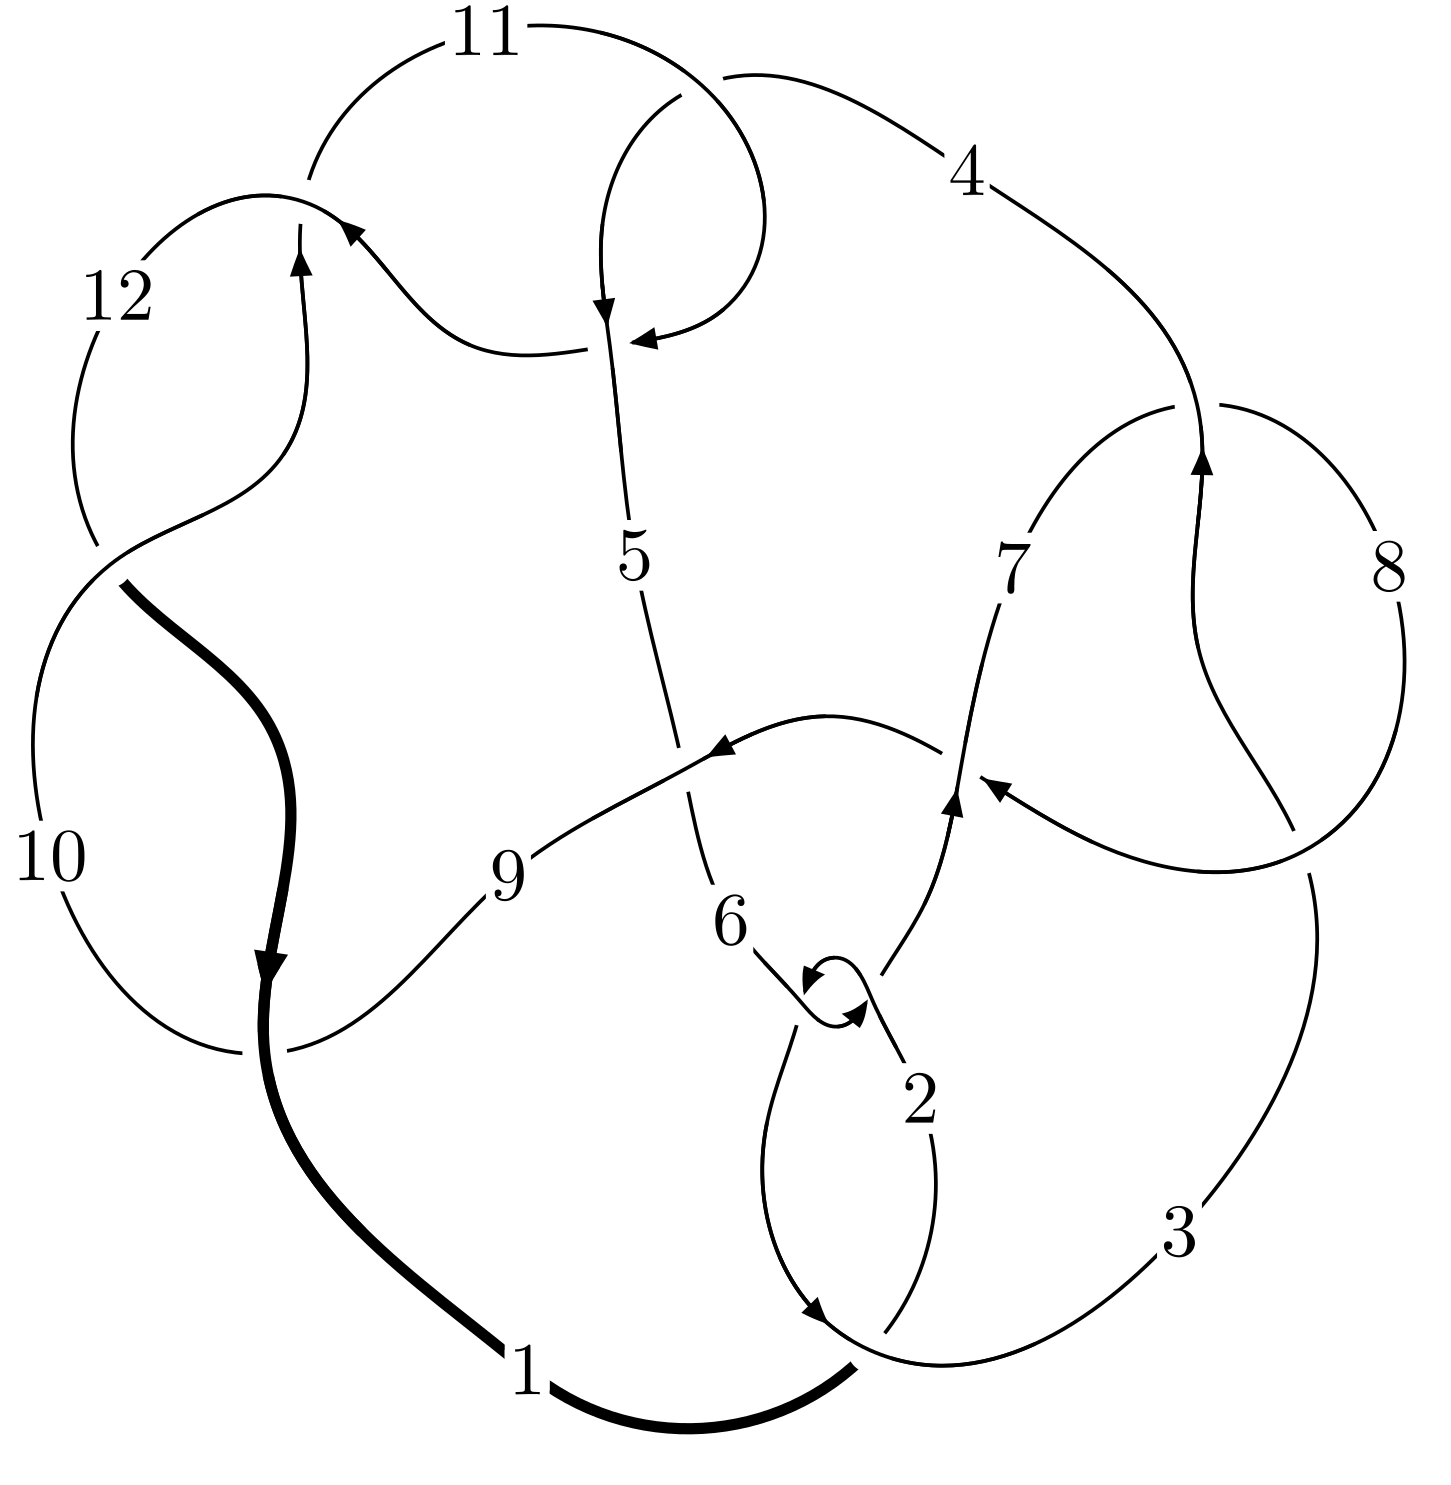
\includegraphics[width=112pt]{../../../GIT/diagram.site/Diagrams/png/1133_12a_0332.png}\\
\ \ \ A knot diagram\footnotemark}&
\allowdisplaybreaks
\textbf{Linearized knot diagam} \\
\cline{2-2}
 &
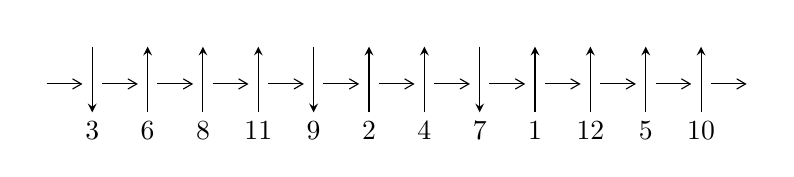
\begin{tikzpicture}[x=20pt, y=17pt]
	% nodes
	\node (C0) at (0, 0) {};
	\node (C1) at (1, 0) {};
	\node (C1U) at (1, +1) {};
	\node (C1D) at (1, -1) {3};

	\node (C2) at (2, 0) {};
	\node (C2U) at (2, +1) {};
	\node (C2D) at (2, -1) {6};

	\node (C3) at (3, 0) {};
	\node (C3U) at (3, +1) {};
	\node (C3D) at (3, -1) {8};

	\node (C4) at (4, 0) {};
	\node (C4U) at (4, +1) {};
	\node (C4D) at (4, -1) {11};

	\node (C5) at (5, 0) {};
	\node (C5U) at (5, +1) {};
	\node (C5D) at (5, -1) {9};

	\node (C6) at (6, 0) {};
	\node (C6U) at (6, +1) {};
	\node (C6D) at (6, -1) {2};

	\node (C7) at (7, 0) {};
	\node (C7U) at (7, +1) {};
	\node (C7D) at (7, -1) {4};

	\node (C8) at (8, 0) {};
	\node (C8U) at (8, +1) {};
	\node (C8D) at (8, -1) {7};

	\node (C9) at (9, 0) {};
	\node (C9U) at (9, +1) {};
	\node (C9D) at (9, -1) {1};

	\node (C10) at (10, 0) {};
	\node (C10U) at (10, +1) {};
	\node (C10D) at (10, -1) {12};

	\node (C11) at (11, 0) {};
	\node (C11U) at (11, +1) {};
	\node (C11D) at (11, -1) {5};

	\node (C12) at (12, 0) {};
	\node (C12U) at (12, +1) {};
	\node (C12D) at (12, -1) {10};
	\node (C13) at (13, 0) {};

	% arrows
	\draw[->,>={angle 60}]
	(C0) edge (C1) (C1) edge (C2) (C2) edge (C3) (C3) edge (C4) (C4) edge (C5) (C5) edge (C6) (C6) edge (C7) (C7) edge (C8) (C8) edge (C9) (C9) edge (C10) (C10) edge (C11) (C11) edge (C12) (C12) edge (C13) ;	\draw[->,>=stealth]
	(C1U) edge (C1D) (C2D) edge (C2U) (C3D) edge (C3U) (C4D) edge (C4U) (C5U) edge (C5D) (C6D) edge (C6U) (C7D) edge (C7U) (C8U) edge (C8D) (C9D) edge (C9U) (C10D) edge (C10U) (C11D) edge (C11U) (C12D) edge (C12U) ;
	\end{tikzpicture} \\
\hhline{~~} \\& 
\textbf{Solving Sequence} \\ \cline{2-2} 
 &
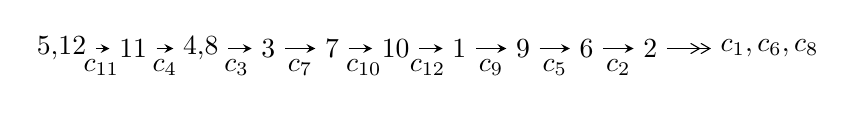
\begin{tikzpicture}[x=23pt, y=7pt]
	% node
	\node (A0) at (-1/8, 0) {5,12};
	\node (A1) at (1, 0) {11};
	\node (A2) at (33/16, 0) {4,8};
	\node (A3) at (25/8, 0) {3};
	\node (A4) at (33/8, 0) {7};
	\node (A5) at (41/8, 0) {10};
	\node (A6) at (49/8, 0) {1};
	\node (A7) at (57/8, 0) {9};
	\node (A8) at (65/8, 0) {6};
	\node (A9) at (73/8, 0) {2};
	\node (C1) at (1/2, -1) {$c_{11}$};
	\node (C2) at (3/2, -1) {$c_{4}$};
	\node (C3) at (21/8, -1) {$c_{3}$};
	\node (C4) at (29/8, -1) {$c_{7}$};
	\node (C5) at (37/8, -1) {$c_{10}$};
	\node (C6) at (45/8, -1) {$c_{12}$};
	\node (C7) at (53/8, -1) {$c_{9}$};
	\node (C8) at (61/8, -1) {$c_{5}$};
	\node (C9) at (69/8, -1) {$c_{2}$};
	\node (A10) at (11, 0) {$c_{1},c_{6},c_{8}$};

	% edge
	\draw[->,>=stealth]	
	(A0) edge (A1) (A1) edge (A2) (A2) edge (A3) (A3) edge (A4) (A4) edge (A5) (A5) edge (A6) (A6) edge (A7) (A7) edge (A8) (A8) edge (A9) ;
	\draw[->>,>={angle 60}]	
	(A9) edge (A10);
\end{tikzpicture} \\ 

\end{tabular} \\

\footnotetext{
The image of knot diagram is generated by the software ``\textbf{Draw programme}" developed by Andrew Bartholomew(\url{http://www.layer8.co.uk/maths/draw/index.htm\#Running-draw}), where we modified some parts for our purpose(\url{https://github.com/CATsTAILs/LinksPainter}).
}\phantom \\ \newline 
\centering \textbf{Ideals for irreducible components\footnotemark of $X_{\text{par}}$} 
 
\begin{align*}
I^u_{1}&=\langle 
- u^{36}+2 u^{35}+\cdots+b+1,\;u^{36}-3 u^{35}+\cdots+2 a-3,\;u^{37}-3 u^{36}+\cdots+u+2\rangle \\
I^u_{2}&=\langle 
- u^{26} a-2 u^{27}+\cdots- a+2,\;2 u^{27} a+2 u^{26} a+\cdots+a^2+1,\;u^{28}+u^{27}+\cdots- u^2+1\rangle \\
I^u_{3}&=\langle 
u^7- u^6- u^5+3 u^3+b- u,\;- u^7+2 u^6+u^5-2 u^4-3 u^3+4 u^2+a+2 u-2,\;u^8- u^6+3 u^4-2 u^2+1\rangle \\
\\
\end{align*}
\raggedright * 3 irreducible components of $\dim_{\mathbb{C}}=0$, with total 101 representations.\\
\footnotetext{All coefficients of polynomials are rational numbers. But the coefficients are sometimes approximated in decimal forms when there is not enough margin.}
\newpage
\renewcommand{\arraystretch}{1}
\centering \section*{I. $I^u_{1}= \langle - u^{36}+2 u^{35}+\cdots+b+1,\;u^{36}-3 u^{35}+\cdots+2 a-3,\;u^{37}-3 u^{36}+\cdots+u+2 \rangle$}
\flushleft \textbf{(i) Arc colorings}\\
\begin{tabular}{m{7pt} m{180pt} m{7pt} m{180pt} }
\flushright $a_{5}=$&$\begin{pmatrix}0\\u\end{pmatrix}$ \\
\flushright $a_{12}=$&$\begin{pmatrix}1\\0\end{pmatrix}$ \\
\flushright $a_{11}=$&$\begin{pmatrix}1\\u^2\end{pmatrix}$ \\
\flushright $a_{4}=$&$\begin{pmatrix}- u\\- u^3+u\end{pmatrix}$ \\
\flushright $a_{8}=$&$\begin{pmatrix}-\frac{1}{2} u^{36}+\frac{3}{2} u^{35}+\cdots+u+\frac{3}{2}\\u^{36}-2 u^{35}+\cdots- u-1\end{pmatrix}$ \\
\flushright $a_{3}=$&$\begin{pmatrix}-\frac{5}{2} u^{36}+\frac{5}{2} u^{35}+\cdots-5 u-\frac{1}{2}\\-2 u^{36}+9 u^{35}+\cdots+13 u+9\end{pmatrix}$ \\
\flushright $a_{7}=$&$\begin{pmatrix}\frac{1}{2} u^{36}-\frac{3}{2} u^{35}+\cdots- u-\frac{1}{2}\\-2 u^{36}+3 u^{35}+\cdots- u+1\end{pmatrix}$ \\
\flushright $a_{10}=$&$\begin{pmatrix}- u^2+1\\u^2\end{pmatrix}$ \\
\flushright $a_{1}=$&$\begin{pmatrix}u^4- u^2+1\\- u^4\end{pmatrix}$ \\
\flushright $a_{9}=$&$\begin{pmatrix}- u^6+u^4-2 u^2+1\\u^6+u^2\end{pmatrix}$ \\
\flushright $a_{6}=$&$\begin{pmatrix}- u^{13}+2 u^{11}-5 u^9+6 u^7-6 u^5+4 u^3- u\\u^{13}- u^{11}+3 u^9-2 u^7+2 u^5- u^3+u\end{pmatrix}$ \\
\flushright $a_{2}=$&$\begin{pmatrix}\frac{3}{2} u^{36}-\frac{3}{2} u^{35}+\cdots+3 u+\frac{3}{2}\\u^{36}-5 u^{35}+\cdots-7 u-5\end{pmatrix}$\\&\end{tabular}
\flushleft \textbf{(ii) Obstruction class $= -1$}\\~\\
\flushleft \textbf{(iii) Cusp Shapes $= -2 u^{36}+12 u^{35}-2 u^{34}-54 u^{33}+30 u^{32}+204 u^{31}-162 u^{30}-520 u^{29}+510 u^{28}+1120 u^{27}-1224 u^{26}-1954 u^{25}+2294 u^{24}+2956 u^{23}-3538 u^{22}-3846 u^{21}+4422 u^{20}+4450 u^{19}-4544 u^{18}-4538 u^{17}+3660 u^{16}+4144 u^{15}-2156 u^{14}-3248 u^{13}+644 u^{12}+2146 u^{11}+292 u^{10}-1052 u^9-570 u^8+292 u^7+378 u^6+46 u^5-134 u^4-70 u^3+4 u^2+26 u+26$}\\~\\
\newpage\renewcommand{\arraystretch}{1}
\flushleft \textbf{(iv) u-Polynomials at the component}\newline \\
\begin{tabular}{m{50pt}|m{274pt}}
Crossings & \hspace{64pt}u-Polynomials at each crossing \\
\hline $$\begin{aligned}c_{1},c_{8}\end{aligned}$$&$\begin{aligned}
&u^{37}+16 u^{36}+\cdots-5 u-1
\end{aligned}$\\
\hline $$\begin{aligned}c_{2},c_{3},c_{6}\\c_{7}\end{aligned}$$&$\begin{aligned}
&u^{37}+8 u^{35}+\cdots+3 u-1
\end{aligned}$\\
\hline $$\begin{aligned}c_{4},c_{11}\end{aligned}$$&$\begin{aligned}
&u^{37}+3 u^{36}+\cdots+u-2
\end{aligned}$\\
\hline $$\begin{aligned}c_{5}\end{aligned}$$&$\begin{aligned}
&u^{37}-21 u^{36}+\cdots+11969 u-898
\end{aligned}$\\
\hline $$\begin{aligned}c_{9},c_{10},c_{12}\end{aligned}$$&$\begin{aligned}
&u^{37}-9 u^{36}+\cdots+9 u-4
\end{aligned}$\\
\hline
\end{tabular}\\~\\
\newpage\renewcommand{\arraystretch}{1}
\flushleft \textbf{(v) Riley Polynomials at the component}\newline \\
\begin{tabular}{m{50pt}|m{274pt}}
Crossings & \hspace{64pt}Riley Polynomials at each crossing \\
\hline $$\begin{aligned}c_{1},c_{8}\end{aligned}$$&$\begin{aligned}
&y^{37}+20 y^{36}+\cdots+83 y-1
\end{aligned}$\\
\hline $$\begin{aligned}c_{2},c_{3},c_{6}\\c_{7}\end{aligned}$$&$\begin{aligned}
&y^{37}+16 y^{36}+\cdots-5 y-1
\end{aligned}$\\
\hline $$\begin{aligned}c_{4},c_{11}\end{aligned}$$&$\begin{aligned}
&y^{37}-9 y^{36}+\cdots+9 y-4
\end{aligned}$\\
\hline $$\begin{aligned}c_{5}\end{aligned}$$&$\begin{aligned}
&y^{37}-9 y^{36}+\cdots+9968617 y-806404
\end{aligned}$\\
\hline $$\begin{aligned}c_{9},c_{10},c_{12}\end{aligned}$$&$\begin{aligned}
&y^{37}+39 y^{36}+\cdots+257 y-16
\end{aligned}$\\
\hline
\end{tabular}\\~\\
\newpage\flushleft \textbf{(vi) Complex Volumes and Cusp Shapes}
$$\begin{array}{c|c|c}  
\text{Solutions to }I^u_{1}& \I (\text{vol} + \sqrt{-1}CS) & \text{Cusp shape}\\
 \hline 
\begin{aligned}
u &= -0.956735 + 0.301871 I \\
a &= \phantom{-}0.107211 + 0.253891 I \\
b &= -0.426927 - 0.834723 I\end{aligned}
 & \phantom{-}4.07996 - 1.69437 I & \phantom{-}12.28632 + 1.79481 I \\ \hline\begin{aligned}
u &= -0.956735 - 0.301871 I \\
a &= \phantom{-}0.107211 - 0.253891 I \\
b &= -0.426927 + 0.834723 I\end{aligned}
 & \phantom{-}4.07996 + 1.69437 I & \phantom{-}12.28632 - 1.79481 I \\ \hline\begin{aligned}
u &= \phantom{-}0.958389 + 0.235458 I \\
a &= -0.753757 + 0.244529 I \\
b &= \phantom{-}0.864634 + 0.110338 I\end{aligned}
 & \phantom{-}4.44965 + 3.84432 I & \phantom{-}12.5649 - 6.9040 I \\ \hline\begin{aligned}
u &= \phantom{-}0.958389 - 0.235458 I \\
a &= -0.753757 - 0.244529 I \\
b &= \phantom{-}0.864634 - 0.110338 I\end{aligned}
 & \phantom{-}4.44965 - 3.84432 I & \phantom{-}12.5649 + 6.9040 I \\ \hline\begin{aligned}
u &= \phantom{-}0.974044 + 0.110846 I \\
a &= \phantom{-}0.438179 + 0.800925 I \\
b &= -0.697177 + 1.212880 I\end{aligned}
 & \phantom{-}1.78420 - 6.55614 I & \phantom{-}9.22168 + 4.71128 I \\ \hline\begin{aligned}
u &= \phantom{-}0.974044 - 0.110846 I \\
a &= \phantom{-}0.438179 - 0.800925 I \\
b &= -0.697177 - 1.212880 I\end{aligned}
 & \phantom{-}1.78420 + 6.55614 I & \phantom{-}9.22168 - 4.71128 I \\ \hline\begin{aligned}
u &= -0.869494 + 0.549252 I \\
a &= \phantom{-}1.04527 + 1.02873 I \\
b &= \phantom{-}0.332238 - 0.481286 I\end{aligned}
 & -2.07404 + 1.88888 I & \phantom{-}3.74513 - 1.47237 I \\ \hline\begin{aligned}
u &= -0.869494 - 0.549252 I \\
a &= \phantom{-}1.04527 - 1.02873 I \\
b &= \phantom{-}0.332238 + 0.481286 I\end{aligned}
 & -2.07404 - 1.88888 I & \phantom{-}3.74513 + 1.47237 I \\ \hline\begin{aligned}
u &= -0.985335 + 0.388773 I \\
a &= -1.78941 - 1.15884 I \\
b &= \phantom{-}0.368742 + 0.784022 I\end{aligned}
 & \phantom{-}0.19576 - 12.29670 I & \phantom{-}5.96416 + 10.82953 I \\ \hline\begin{aligned}
u &= -0.985335 - 0.388773 I \\
a &= -1.78941 + 1.15884 I \\
b &= \phantom{-}0.368742 - 0.784022 I\end{aligned}
 & \phantom{-}0.19576 + 12.29670 I & \phantom{-}5.96416 - 10.82953 I\\
 \hline 
 \end{array}$$\newpage$$\begin{array}{c|c|c}  
\text{Solutions to }I^u_{1}& \I (\text{vol} + \sqrt{-1}CS) & \text{Cusp shape}\\
 \hline 
\begin{aligned}
u &= -0.806001 + 0.770895 I \\
a &= \phantom{-}0.69552 + 1.27487 I \\
b &= \phantom{-}0.833243 - 1.116330 I\end{aligned}
 & -1.90734 + 2.28917 I & \phantom{-}4.88020 - 3.21889 I \\ \hline\begin{aligned}
u &= -0.806001 - 0.770895 I \\
a &= \phantom{-}0.69552 - 1.27487 I \\
b &= \phantom{-}0.833243 + 1.116330 I\end{aligned}
 & -1.90734 - 2.28917 I & \phantom{-}4.88020 + 3.21889 I \\ \hline\begin{aligned}
u &= \phantom{-}0.695248 + 0.472483 I \\
a &= \phantom{-}0.444025 - 1.024300 I \\
b &= -0.122253 + 0.573991 I\end{aligned}
 & -1.19445 + 1.82713 I & \phantom{-}4.12966 - 6.04101 I \\ \hline\begin{aligned}
u &= \phantom{-}0.695248 - 0.472483 I \\
a &= \phantom{-}0.444025 + 1.024300 I \\
b &= -0.122253 - 0.573991 I\end{aligned}
 & -1.19445 - 1.82713 I & \phantom{-}4.12966 + 6.04101 I \\ \hline\begin{aligned}
u &= \phantom{-}0.826193 + 0.842773 I \\
a &= -0.567500 - 0.335315 I \\
b &= \phantom{-}0.360895 - 0.189373 I\end{aligned}
 & -3.16743 + 0.36820 I & \phantom{-}6.31788 - 2.12826 I \\ \hline\begin{aligned}
u &= \phantom{-}0.826193 - 0.842773 I \\
a &= -0.567500 + 0.335315 I \\
b &= \phantom{-}0.360895 + 0.189373 I\end{aligned}
 & -3.16743 - 0.36820 I & \phantom{-}6.31788 + 2.12826 I \\ \hline\begin{aligned}
u &= -0.492238 + 0.655396 I \\
a &= \phantom{-}0.068505 + 1.209380 I \\
b &= -0.723783 - 1.213940 I\end{aligned}
 & -3.23955 - 6.28444 I & \phantom{-}0.23042 + 7.24447 I \\ \hline\begin{aligned}
u &= -0.492238 - 0.655396 I \\
a &= \phantom{-}0.068505 - 1.209380 I \\
b &= -0.723783 + 1.213940 I\end{aligned}
 & -3.23955 + 6.28444 I & \phantom{-}0.23042 - 7.24447 I \\ \hline\begin{aligned}
u &= -0.942981 + 0.761048 I \\
a &= \phantom{-}1.151510 + 0.744837 I \\
b &= -0.60571 - 2.01178 I\end{aligned}
 & -1.50596 - 8.08923 I & \phantom{-}6.07656 + 8.51523 I \\ \hline\begin{aligned}
u &= -0.942981 - 0.761048 I \\
a &= \phantom{-}1.151510 - 0.744837 I \\
b &= -0.60571 + 2.01178 I\end{aligned}
 & -1.50596 + 8.08923 I & \phantom{-}6.07656 - 8.51523 I\\
 \hline 
 \end{array}$$\newpage$$\begin{array}{c|c|c}  
\text{Solutions to }I^u_{1}& \I (\text{vol} + \sqrt{-1}CS) & \text{Cusp shape}\\
 \hline 
\begin{aligned}
u &= \phantom{-}0.827155 + 0.889743 I \\
a &= \phantom{-}1.41124 - 2.73920 I \\
b &= \phantom{-}2.08237 + 4.08970 I\end{aligned}
 & -8.12556 - 10.18450 I & \phantom{-}0.37161 + 5.66795 I \\ \hline\begin{aligned}
u &= \phantom{-}0.827155 - 0.889743 I \\
a &= \phantom{-}1.41124 + 2.73920 I \\
b &= \phantom{-}2.08237 - 4.08970 I\end{aligned}
 & -8.12556 + 10.18450 I & \phantom{-}0.37161 - 5.66795 I \\ \hline\begin{aligned}
u &= \phantom{-}0.960937 + 0.799626 I \\
a &= \phantom{-}0.367828 + 0.480609 I \\
b &= -0.706212 - 0.437969 I\end{aligned}
 & -2.75006 + 5.76064 I & \phantom{-}7.04693 - 2.89668 I \\ \hline\begin{aligned}
u &= \phantom{-}0.960937 - 0.799626 I \\
a &= \phantom{-}0.367828 - 0.480609 I \\
b &= -0.706212 + 0.437969 I\end{aligned}
 & -2.75006 - 5.76064 I & \phantom{-}7.04693 + 2.89668 I \\ \hline\begin{aligned}
u &= \phantom{-}0.888234 + 0.886878 I \\
a &= -1.24637 + 2.29159 I \\
b &= -1.53871 - 3.88705 I\end{aligned}
 & -10.85650 + 5.89802 I & -1.00813 - 7.72734 I \\ \hline\begin{aligned}
u &= \phantom{-}0.888234 - 0.886878 I \\
a &= -1.24637 - 2.29159 I \\
b &= -1.53871 + 3.88705 I\end{aligned}
 & -10.85650 - 5.89802 I & -1.00813 + 7.72734 I \\ \hline\begin{aligned}
u &= -0.916359 + 0.865710 I \\
a &= -1.40408 - 1.51780 I \\
b &= -0.73441 + 3.20038 I\end{aligned}
 & -8.85573 - 3.20735 I & \phantom{-}5.22275 + 2.78415 I \\ \hline\begin{aligned}
u &= -0.916359 - 0.865710 I \\
a &= -1.40408 + 1.51780 I \\
b &= -0.73441 - 3.20038 I\end{aligned}
 & -8.85573 + 3.20735 I & \phantom{-}5.22275 - 2.78415 I \\ \hline\begin{aligned}
u &= \phantom{-}0.947451 + 0.860827 I \\
a &= -2.19419 + 1.40646 I \\
b &= -0.12980 - 3.94938 I\end{aligned}
 & -10.66820 + 0.56453 I & -0.58196 + 3.04417 I \\ \hline\begin{aligned}
u &= \phantom{-}0.947451 - 0.860827 I \\
a &= -2.19419 - 1.40646 I \\
b &= -0.12980 + 3.94938 I\end{aligned}
 & -10.66820 - 0.56453 I & -0.58196 - 3.04417 I\\
 \hline 
 \end{array}$$\newpage$$\begin{array}{c|c|c}  
\text{Solutions to }I^u_{1}& \I (\text{vol} + \sqrt{-1}CS) & \text{Cusp shape}\\
 \hline 
\begin{aligned}
u &= \phantom{-}0.983458 + 0.824484 I \\
a &= \phantom{-}2.65593 - 1.57243 I \\
b &= -0.29611 + 5.01537 I\end{aligned}
 & -7.6317 + 16.5331 I & \phantom{-}1.29247 - 10.38801 I \\ \hline\begin{aligned}
u &= \phantom{-}0.983458 - 0.824484 I \\
a &= \phantom{-}2.65593 + 1.57243 I \\
b &= -0.29611 - 5.01537 I\end{aligned}
 & -7.6317 - 16.5331 I & \phantom{-}1.29247 + 10.38801 I \\ \hline\begin{aligned}
u &= -0.240182 + 0.666603 I \\
a &= -0.12252 - 1.87056 I \\
b &= \phantom{-}0.79192 + 1.32245 I\end{aligned}
 & -2.16954 + 8.48653 I & \phantom{-}0.54078 - 6.28516 I \\ \hline\begin{aligned}
u &= -0.240182 - 0.666603 I \\
a &= -0.12252 + 1.87056 I \\
b &= \phantom{-}0.79192 - 1.32245 I\end{aligned}
 & -2.16954 - 8.48653 I & \phantom{-}0.54078 + 6.28516 I \\ \hline\begin{aligned}
u &= -0.595207\phantom{ +0.000000I} \\
a &= \phantom{-}0.354844\phantom{ +0.000000I} \\
b &= \phantom{-}0.343586\phantom{ +0.000000I}\end{aligned}
 & \phantom{-}0.761151\phantom{ +0.000000I} & \phantom{-}13.8790\phantom{ +0.000000I} \\ \hline\begin{aligned}
u &= -0.054179 + 0.561331 I \\
a &= \phantom{-}0.765177 + 0.865041 I \\
b &= \phantom{-}0.175261 - 0.166101 I\end{aligned}
 & \phantom{-}1.44057 - 1.28380 I & \phantom{-}5.75923 + 3.39663 I \\ \hline\begin{aligned}
u &= -0.054179 - 0.561331 I \\
a &= \phantom{-}0.765177 - 0.865041 I \\
b &= \phantom{-}0.175261 + 0.166101 I\end{aligned}
 & \phantom{-}1.44057 + 1.28380 I & \phantom{-}5.75923 - 3.39663 I\\
 \hline 
 \end{array}$$\newpage\newpage\renewcommand{\arraystretch}{1}
\centering \section*{II. $I^u_{2}= \langle - u^{26} a-2 u^{27}+\cdots- a+2,\;2 u^{27} a+2 u^{26} a+\cdots+a^2+1,\;u^{28}+u^{27}+\cdots- u^2+1 \rangle$}
\flushleft \textbf{(i) Arc colorings}\\
\begin{tabular}{m{7pt} m{180pt} m{7pt} m{180pt} }
\flushright $a_{5}=$&$\begin{pmatrix}0\\u\end{pmatrix}$ \\
\flushright $a_{12}=$&$\begin{pmatrix}1\\0\end{pmatrix}$ \\
\flushright $a_{11}=$&$\begin{pmatrix}1\\u^2\end{pmatrix}$ \\
\flushright $a_{4}=$&$\begin{pmatrix}- u\\- u^3+u\end{pmatrix}$ \\
\flushright $a_{8}=$&$\begin{pmatrix}a\\u^{26} a+2 u^{27}+\cdots+a-2\end{pmatrix}$ \\
\flushright $a_{3}=$&$\begin{pmatrix}-2 u^{27}-3 u^{26}+\cdots-2 a+1\\2 u^{25} a+2 u^{24} a+\cdots+2 a u-1\end{pmatrix}$ \\
\flushright $a_{7}=$&$\begin{pmatrix}-2 u^{27} a-4 u^{26} a+\cdots+2 a+2 u\\2 u^{27} a+4 u^{27}+\cdots+2 a-4\end{pmatrix}$ \\
\flushright $a_{10}=$&$\begin{pmatrix}- u^2+1\\u^2\end{pmatrix}$ \\
\flushright $a_{1}=$&$\begin{pmatrix}u^4- u^2+1\\- u^4\end{pmatrix}$ \\
\flushright $a_{9}=$&$\begin{pmatrix}- u^6+u^4-2 u^2+1\\u^6+u^2\end{pmatrix}$ \\
\flushright $a_{6}=$&$\begin{pmatrix}- u^{13}+2 u^{11}-5 u^9+6 u^7-6 u^5+4 u^3- u\\u^{13}- u^{11}+3 u^9-2 u^7+2 u^5- u^3+u\end{pmatrix}$ \\
\flushright $a_{2}=$&$\begin{pmatrix}-2 u^{27}-2 u^{26}+\cdots-2 a+2\\-2 u^{27} a-4 u^{26} a+\cdots+2 a-2\end{pmatrix}$\\&\end{tabular}
\flushleft \textbf{(ii) Obstruction class $= -1$}\\~\\
\flushleft \textbf{(iii) Cusp Shapes $= -4 u^{26}-4 u^{25}+12 u^{24}+16 u^{23}-44 u^{22}-52 u^{21}+88 u^{20}+116 u^{19}-168 u^{18}-204 u^{17}+236 u^{16}+284 u^{15}-288 u^{14}-312 u^{13}+280 u^{12}+256 u^{11}-224 u^{10}-152 u^9+136 u^8+40 u^7-64 u^6+16 u^5+16 u^4-16 u^3+4 u+6$}\\~\\
\newpage\renewcommand{\arraystretch}{1}
\flushleft \textbf{(iv) u-Polynomials at the component}\newline \\
\begin{tabular}{m{50pt}|m{274pt}}
Crossings & \hspace{64pt}u-Polynomials at each crossing \\
\hline $$\begin{aligned}c_{1},c_{8}\end{aligned}$$&$\begin{aligned}
&u^{56}+31 u^{55}+\cdots+27 u+4
\end{aligned}$\\
\hline $$\begin{aligned}c_{2},c_{3},c_{6}\\c_{7}\end{aligned}$$&$\begin{aligned}
&u^{56}- u^{55}+\cdots+u+2
\end{aligned}$\\
\hline $$\begin{aligned}c_{4},c_{11}\end{aligned}$$&$\begin{aligned}
&(u^{28}- u^{27}+\cdots- u^2+1)^{2}
\end{aligned}$\\
\hline $$\begin{aligned}c_{5}\end{aligned}$$&$\begin{aligned}
&(u^{28}+7 u^{27}+\cdots+8 u+1)^{2}
\end{aligned}$\\
\hline $$\begin{aligned}c_{9},c_{10},c_{12}\end{aligned}$$&$\begin{aligned}
&(u^{28}-7 u^{27}+\cdots-2 u+1)^{2}
\end{aligned}$\\
\hline
\end{tabular}\\~\\
\newpage\renewcommand{\arraystretch}{1}
\flushleft \textbf{(v) Riley Polynomials at the component}\newline \\
\begin{tabular}{m{50pt}|m{274pt}}
Crossings & \hspace{64pt}Riley Polynomials at each crossing \\
\hline $$\begin{aligned}c_{1},c_{8}\end{aligned}$$&$\begin{aligned}
&y^{56}-13 y^{55}+\cdots+927 y+16
\end{aligned}$\\
\hline $$\begin{aligned}c_{2},c_{3},c_{6}\\c_{7}\end{aligned}$$&$\begin{aligned}
&y^{56}+31 y^{55}+\cdots+27 y+4
\end{aligned}$\\
\hline $$\begin{aligned}c_{4},c_{11}\end{aligned}$$&$\begin{aligned}
&(y^{28}-7 y^{27}+\cdots-2 y+1)^{2}
\end{aligned}$\\
\hline $$\begin{aligned}c_{5}\end{aligned}$$&$\begin{aligned}
&(y^{28}+y^{27}+\cdots+62 y+1)^{2}
\end{aligned}$\\
\hline $$\begin{aligned}c_{9},c_{10},c_{12}\end{aligned}$$&$\begin{aligned}
&(y^{28}+29 y^{27}+\cdots+14 y+1)^{2}
\end{aligned}$\\
\hline
\end{tabular}\\~\\
\newpage\flushleft \textbf{(vi) Complex Volumes and Cusp Shapes}
$$\begin{array}{c|c|c}  
\text{Solutions to }I^u_{2}& \I (\text{vol} + \sqrt{-1}CS) & \text{Cusp shape}\\
 \hline 
\begin{aligned}
u &= -0.899770 + 0.359295 I \\
a &= \phantom{-}1.02424 + 1.44935 I \\
b &= \phantom{-}0.317596 + 0.143962 I\end{aligned}
 & -2.76021 - 3.76187 I & \phantom{-}4.54869 + 7.99757 I \\ \hline\begin{aligned}
u &= -0.899770 + 0.359295 I \\
a &= -2.28758 - 0.15491 I \\
b &= \phantom{-}1.40296 + 0.75227 I\end{aligned}
 & -2.76021 - 3.76187 I & \phantom{-}4.54869 + 7.99757 I \\ \hline\begin{aligned}
u &= -0.899770 - 0.359295 I \\
a &= \phantom{-}1.02424 - 1.44935 I \\
b &= \phantom{-}0.317596 - 0.143962 I\end{aligned}
 & -2.76021 + 3.76187 I & \phantom{-}4.54869 - 7.99757 I \\ \hline\begin{aligned}
u &= -0.899770 - 0.359295 I \\
a &= -2.28758 + 0.15491 I \\
b &= \phantom{-}1.40296 - 0.75227 I\end{aligned}
 & -2.76021 + 3.76187 I & \phantom{-}4.54869 - 7.99757 I \\ \hline\begin{aligned}
u &= -0.954301 + 0.165131 I \\
a &= \phantom{-}0.453330 - 0.469903 I \\
b &= -0.670608 - 1.151640 I\end{aligned}
 & \phantom{-}3.64668 + 1.29573 I & \phantom{-}12.16340 + 0.19021 I \\ \hline\begin{aligned}
u &= -0.954301 + 0.165131 I \\
a &= -0.381153 - 0.148423 I \\
b &= \phantom{-}0.877426 - 0.189403 I\end{aligned}
 & \phantom{-}3.64668 + 1.29573 I & \phantom{-}12.16340 + 0.19021 I \\ \hline\begin{aligned}
u &= -0.954301 - 0.165131 I \\
a &= \phantom{-}0.453330 + 0.469903 I \\
b &= -0.670608 + 1.151640 I\end{aligned}
 & \phantom{-}3.64668 - 1.29573 I & \phantom{-}12.16340 - 0.19021 I \\ \hline\begin{aligned}
u &= -0.954301 - 0.165131 I \\
a &= -0.381153 + 0.148423 I \\
b &= \phantom{-}0.877426 + 0.189403 I\end{aligned}
 & \phantom{-}3.64668 - 1.29573 I & \phantom{-}12.16340 - 0.19021 I \\ \hline\begin{aligned}
u &= \phantom{-}0.971170 + 0.356128 I \\
a &= -0.056263 - 0.455331 I \\
b &= -0.331645 + 0.653502 I\end{aligned}
 & \phantom{-}2.55576 + 6.87695 I & \phantom{-}9.38448 - 7.29150 I \\ \hline\begin{aligned}
u &= \phantom{-}0.971170 + 0.356128 I \\
a &= -1.66109 + 0.82974 I \\
b &= \phantom{-}0.635990 - 0.561304 I\end{aligned}
 & \phantom{-}2.55576 + 6.87695 I & \phantom{-}9.38448 - 7.29150 I\\
 \hline 
 \end{array}$$\newpage$$\begin{array}{c|c|c}  
\text{Solutions to }I^u_{2}& \I (\text{vol} + \sqrt{-1}CS) & \text{Cusp shape}\\
 \hline 
\begin{aligned}
u &= \phantom{-}0.971170 - 0.356128 I \\
a &= -0.056263 + 0.455331 I \\
b &= -0.331645 - 0.653502 I\end{aligned}
 & \phantom{-}2.55576 - 6.87695 I & \phantom{-}9.38448 + 7.29150 I \\ \hline\begin{aligned}
u &= \phantom{-}0.971170 - 0.356128 I \\
a &= -1.66109 - 0.82974 I \\
b &= \phantom{-}0.635990 + 0.561304 I\end{aligned}
 & \phantom{-}2.55576 - 6.87695 I & \phantom{-}9.38448 + 7.29150 I \\ \hline\begin{aligned}
u &= \phantom{-}0.816311 + 0.219669 I \\
a &= \phantom{-}1.44748 - 0.37350 I \\
b &= -0.48686 + 1.64839 I\end{aligned}
 & -1.87609 + 0.68499 I & \phantom{-}8.66956 - 0.56233 I \\ \hline\begin{aligned}
u &= \phantom{-}0.816311 + 0.219669 I \\
a &= \phantom{-}0.89236 - 1.56400 I \\
b &= -0.222133 - 0.418971 I\end{aligned}
 & -1.87609 + 0.68499 I & \phantom{-}8.66956 - 0.56233 I \\ \hline\begin{aligned}
u &= \phantom{-}0.816311 - 0.219669 I \\
a &= \phantom{-}1.44748 + 0.37350 I \\
b &= -0.48686 - 1.64839 I\end{aligned}
 & -1.87609 - 0.68499 I & \phantom{-}8.66956 + 0.56233 I \\ \hline\begin{aligned}
u &= \phantom{-}0.816311 - 0.219669 I \\
a &= \phantom{-}0.89236 + 1.56400 I \\
b &= -0.222133 + 0.418971 I\end{aligned}
 & -1.87609 - 0.68499 I & \phantom{-}8.66956 + 0.56233 I \\ \hline\begin{aligned}
u &= \phantom{-}0.894569 + 0.739690 I \\
a &= \phantom{-}0.546052 - 0.607895 I \\
b &= -0.438838 + 1.131330 I\end{aligned}
 & -1.35470 + 2.81005 I & \phantom{-}6.61718 - 2.93426 I \\ \hline\begin{aligned}
u &= \phantom{-}0.894569 + 0.739690 I \\
a &= \phantom{-}0.522067 - 0.615995 I \\
b &= \phantom{-}0.467816 + 0.278002 I\end{aligned}
 & -1.35470 + 2.81005 I & \phantom{-}6.61718 - 2.93426 I \\ \hline\begin{aligned}
u &= \phantom{-}0.894569 - 0.739690 I \\
a &= \phantom{-}0.546052 + 0.607895 I \\
b &= -0.438838 - 1.131330 I\end{aligned}
 & -1.35470 - 2.81005 I & \phantom{-}6.61718 + 2.93426 I \\ \hline\begin{aligned}
u &= \phantom{-}0.894569 - 0.739690 I \\
a &= \phantom{-}0.522067 + 0.615995 I \\
b &= \phantom{-}0.467816 - 0.278002 I\end{aligned}
 & -1.35470 - 2.81005 I & \phantom{-}6.61718 + 2.93426 I\\
 \hline 
 \end{array}$$\newpage$$\begin{array}{c|c|c}  
\text{Solutions to }I^u_{2}& \I (\text{vol} + \sqrt{-1}CS) & \text{Cusp shape}\\
 \hline 
\begin{aligned}
u &= \phantom{-}0.594944 + 0.540484 I \\
a &= \phantom{-}0.796189 - 0.763146 I \\
b &= -0.123628 + 0.489316 I\end{aligned}
 & -1.33499 + 1.97473 I & \phantom{-}3.44037 - 3.90307 I \\ \hline\begin{aligned}
u &= \phantom{-}0.594944 + 0.540484 I \\
a &= \phantom{-}0.187055 - 1.218540 I \\
b &= -0.446420 + 0.779097 I\end{aligned}
 & -1.33499 + 1.97473 I & \phantom{-}3.44037 - 3.90307 I \\ \hline\begin{aligned}
u &= \phantom{-}0.594944 - 0.540484 I \\
a &= \phantom{-}0.796189 + 0.763146 I \\
b &= -0.123628 - 0.489316 I\end{aligned}
 & -1.33499 - 1.97473 I & \phantom{-}3.44037 + 3.90307 I \\ \hline\begin{aligned}
u &= \phantom{-}0.594944 - 0.540484 I \\
a &= \phantom{-}0.187055 + 1.218540 I \\
b &= -0.446420 - 0.779097 I\end{aligned}
 & -1.33499 - 1.97473 I & \phantom{-}3.44037 + 3.90307 I \\ \hline\begin{aligned}
u &= -0.824272 + 0.873080 I \\
a &= -0.868359 + 0.410750 I \\
b &= \phantom{-}0.860810 + 0.419716 I\end{aligned}
 & -5.36393 + 4.77850 I & \phantom{-}3.36601 - 2.38985 I \\ \hline\begin{aligned}
u &= -0.824272 + 0.873080 I \\
a &= \phantom{-}1.10511 + 2.56923 I \\
b &= \phantom{-}2.16209 - 3.37931 I\end{aligned}
 & -5.36393 + 4.77850 I & \phantom{-}3.36601 - 2.38985 I \\ \hline\begin{aligned}
u &= -0.824272 - 0.873080 I \\
a &= -0.868359 - 0.410750 I \\
b &= \phantom{-}0.860810 - 0.419716 I\end{aligned}
 & -5.36393 - 4.77850 I & \phantom{-}3.36601 + 2.38985 I \\ \hline\begin{aligned}
u &= -0.824272 - 0.873080 I \\
a &= \phantom{-}1.10511 - 2.56923 I \\
b &= \phantom{-}2.16209 + 3.37931 I\end{aligned}
 & -5.36393 - 4.77850 I & \phantom{-}3.36601 + 2.38985 I \\ \hline\begin{aligned}
u &= \phantom{-}0.848977 + 0.862822 I \\
a &= -1.61944 + 2.47231 I \\
b &= -1.04855 - 4.31824 I\end{aligned}
 & -10.42220 - 0.98573 I & -1.20004 + 1.21736 I \\ \hline\begin{aligned}
u &= \phantom{-}0.848977 + 0.862822 I \\
a &= \phantom{-}0.52453 - 2.98229 I \\
b &= \phantom{-}3.47400 + 2.91986 I\end{aligned}
 & -10.42220 - 0.98573 I & -1.20004 + 1.21736 I\\
 \hline 
 \end{array}$$\newpage$$\begin{array}{c|c|c}  
\text{Solutions to }I^u_{2}& \I (\text{vol} + \sqrt{-1}CS) & \text{Cusp shape}\\
 \hline 
\begin{aligned}
u &= \phantom{-}0.848977 - 0.862822 I \\
a &= -1.61944 - 2.47231 I \\
b &= -1.04855 + 4.31824 I\end{aligned}
 & -10.42220 + 0.98573 I & -1.20004 - 1.21736 I \\ \hline\begin{aligned}
u &= \phantom{-}0.848977 - 0.862822 I \\
a &= \phantom{-}0.52453 + 2.98229 I \\
b &= \phantom{-}3.47400 - 2.91986 I\end{aligned}
 & -10.42220 + 0.98573 I & -1.20004 - 1.21736 I \\ \hline\begin{aligned}
u &= -0.883885 + 0.841772 I \\
a &= -0.579421 - 0.504600 I \\
b &= -0.614694 + 1.257450 I\end{aligned}
 & -8.24265 - 2.93440 I & \phantom{-}1.90343 + 3.53352 I \\ \hline\begin{aligned}
u &= -0.883885 + 0.841772 I \\
a &= -1.73296 - 2.18260 I \\
b &= -0.90166 + 3.97609 I\end{aligned}
 & -8.24265 - 2.93440 I & \phantom{-}1.90343 + 3.53352 I \\ \hline\begin{aligned}
u &= -0.883885 - 0.841772 I \\
a &= -0.579421 + 0.504600 I \\
b &= -0.614694 - 1.257450 I\end{aligned}
 & -8.24265 + 2.93440 I & \phantom{-}1.90343 - 3.53352 I \\ \hline\begin{aligned}
u &= -0.883885 - 0.841772 I \\
a &= -1.73296 + 2.18260 I \\
b &= -0.90166 - 3.97609 I\end{aligned}
 & -8.24265 + 2.93440 I & \phantom{-}1.90343 - 3.53352 I \\ \hline\begin{aligned}
u &= -0.921489 + 0.824235 I \\
a &= -0.547487 - 0.474537 I \\
b &= -0.21718 + 1.66408 I\end{aligned}
 & -8.12146 - 3.27187 I & \phantom{-}2.26749 + 1.59380 I \\ \hline\begin{aligned}
u &= -0.921489 + 0.824235 I \\
a &= -2.04938 - 1.94889 I \\
b &= -0.66887 + 3.95674 I\end{aligned}
 & -8.12146 - 3.27187 I & \phantom{-}2.26749 + 1.59380 I \\ \hline\begin{aligned}
u &= -0.921489 - 0.824235 I \\
a &= -0.547487 + 0.474537 I \\
b &= -0.21718 - 1.66408 I\end{aligned}
 & -8.12146 + 3.27187 I & \phantom{-}2.26749 - 1.59380 I \\ \hline\begin{aligned}
u &= -0.921489 - 0.824235 I \\
a &= -2.04938 + 1.94889 I \\
b &= -0.66887 - 3.95674 I\end{aligned}
 & -8.12146 + 3.27187 I & \phantom{-}2.26749 - 1.59380 I\\
 \hline 
 \end{array}$$\newpage$$\begin{array}{c|c|c}  
\text{Solutions to }I^u_{2}& \I (\text{vol} + \sqrt{-1}CS) & \text{Cusp shape}\\
 \hline 
\begin{aligned}
u &= \phantom{-}0.956709 + 0.821698 I \\
a &= \phantom{-}2.87664 - 0.62418 I \\
b &= -2.04478 + 4.61109 I\end{aligned}
 & -10.08390 + 7.24627 I & -0.35343 - 6.30493 I \\ \hline\begin{aligned}
u &= \phantom{-}0.956709 + 0.821698 I \\
a &= -2.34992 + 1.84192 I \\
b &= -0.59666 - 4.17927 I\end{aligned}
 & -10.08390 + 7.24627 I & -0.35343 - 6.30493 I \\ \hline\begin{aligned}
u &= \phantom{-}0.956709 - 0.821698 I \\
a &= \phantom{-}2.87664 + 0.62418 I \\
b &= -2.04478 - 4.61109 I\end{aligned}
 & -10.08390 - 7.24627 I & -0.35343 + 6.30493 I \\ \hline\begin{aligned}
u &= \phantom{-}0.956709 - 0.821698 I \\
a &= -2.34992 - 1.84192 I \\
b &= -0.59666 + 4.17927 I\end{aligned}
 & -10.08390 - 7.24627 I & -0.35343 + 6.30493 I \\ \hline\begin{aligned}
u &= -0.975960 + 0.814541 I \\
a &= \phantom{-}0.461489 - 0.788364 I \\
b &= -1.176520 + 0.452581 I\end{aligned}
 & -4.88826 - 11.04430 I & \phantom{-}4.28365 + 7.20583 I \\ \hline\begin{aligned}
u &= -0.975960 + 0.814541 I \\
a &= \phantom{-}2.47158 + 1.26067 I \\
b &= -0.68026 - 4.45661 I\end{aligned}
 & -4.88826 - 11.04430 I & \phantom{-}4.28365 + 7.20583 I \\ \hline\begin{aligned}
u &= -0.975960 - 0.814541 I \\
a &= \phantom{-}0.461489 + 0.788364 I \\
b &= -1.176520 - 0.452581 I\end{aligned}
 & -4.88826 + 11.04430 I & \phantom{-}4.28365 - 7.20583 I \\ \hline\begin{aligned}
u &= -0.975960 - 0.814541 I \\
a &= \phantom{-}2.47158 - 1.26067 I \\
b &= -0.68026 + 4.45661 I\end{aligned}
 & -4.88826 + 11.04430 I & \phantom{-}4.28365 - 7.20583 I \\ \hline\begin{aligned}
u &= \phantom{-}0.190095 + 0.611771 I \\
a &= \phantom{-}0.740553 - 0.573961 I \\
b &= \phantom{-}0.0110804 - 0.0583490 I\end{aligned}
 & \phantom{-}0.14328 - 3.38176 I & \phantom{-}3.65042 + 2.75424 I \\ \hline\begin{aligned}
u &= \phantom{-}0.190095 + 0.611771 I \\
a &= \phantom{-}0.25617 + 1.77312 I \\
b &= \phantom{-}0.491611 - 1.016080 I\end{aligned}
 & \phantom{-}0.14328 - 3.38176 I & \phantom{-}3.65042 + 2.75424 I\\
 \hline 
 \end{array}$$\newpage$$\begin{array}{c|c|c}  
\text{Solutions to }I^u_{2}& \I (\text{vol} + \sqrt{-1}CS) & \text{Cusp shape}\\
 \hline 
\begin{aligned}
u &= \phantom{-}0.190095 - 0.611771 I \\
a &= \phantom{-}0.740553 + 0.573961 I \\
b &= \phantom{-}0.0110804 + 0.0583490 I\end{aligned}
 & \phantom{-}0.14328 + 3.38176 I & \phantom{-}3.65042 - 2.75424 I \\ \hline\begin{aligned}
u &= \phantom{-}0.190095 - 0.611771 I \\
a &= \phantom{-}0.25617 - 1.77312 I \\
b &= \phantom{-}0.491611 + 1.016080 I\end{aligned}
 & \phantom{-}0.14328 + 3.38176 I & \phantom{-}3.65042 - 2.75424 I \\ \hline\begin{aligned}
u &= -0.313097 + 0.488114 I \\
a &= -0.290579 + 1.243310 I \\
b &= -1.211500 - 0.586102 I\end{aligned}
 & -4.53523 + 0.50746 I & -2.74123 - 1.23953 I \\ \hline\begin{aligned}
u &= -0.313097 + 0.488114 I \\
a &= \phantom{-}0.61878 - 2.72822 I \\
b &= -0.32060 + 1.46145 I\end{aligned}
 & -4.53523 + 0.50746 I & -2.74123 - 1.23953 I \\ \hline\begin{aligned}
u &= -0.313097 - 0.488114 I \\
a &= -0.290579 - 1.243310 I \\
b &= -1.211500 + 0.586102 I\end{aligned}
 & -4.53523 - 0.50746 I & -2.74123 + 1.23953 I \\ \hline\begin{aligned}
u &= -0.313097 - 0.488114 I \\
a &= \phantom{-}0.61878 + 2.72822 I \\
b &= -0.32060 - 1.46145 I\end{aligned}
 & -4.53523 - 0.50746 I & -2.74123 + 1.23953 I\\
 \hline 
 \end{array}$$\newpage\newpage\renewcommand{\arraystretch}{1}
\centering \section*{III. $I^u_{3}= \langle u^7- u^6- u^5+3 u^3+b- u,\;- u^7+2 u^6+\cdots+a-2,\;u^8- u^6+3 u^4-2 u^2+1 \rangle$}
\flushleft \textbf{(i) Arc colorings}\\
\begin{tabular}{m{7pt} m{180pt} m{7pt} m{180pt} }
\flushright $a_{5}=$&$\begin{pmatrix}0\\u\end{pmatrix}$ \\
\flushright $a_{12}=$&$\begin{pmatrix}1\\0\end{pmatrix}$ \\
\flushright $a_{11}=$&$\begin{pmatrix}1\\u^2\end{pmatrix}$ \\
\flushright $a_{4}=$&$\begin{pmatrix}- u\\- u^3+u\end{pmatrix}$ \\
\flushright $a_{8}=$&$\begin{pmatrix}u^7-2 u^6- u^5+2 u^4+3 u^3-4 u^2-2 u+2\\- u^7+u^6+u^5-3 u^3+u\end{pmatrix}$ \\
\flushright $a_{3}=$&$\begin{pmatrix}- u^6-2 u^2+u\\- u^7+u^5+u^4-2 u^3+u+1\end{pmatrix}$ \\
\flushright $a_{7}=$&$\begin{pmatrix}u^7- u^6- u^5+u^4+3 u^3-2 u^2-2 u+1\\- u^7+u^5-3 u^3- u^2+u\end{pmatrix}$ \\
\flushright $a_{10}=$&$\begin{pmatrix}- u^2+1\\u^2\end{pmatrix}$ \\
\flushright $a_{1}=$&$\begin{pmatrix}u^4- u^2+1\\- u^4\end{pmatrix}$ \\
\flushright $a_{9}=$&$\begin{pmatrix}- u^6+u^4-2 u^2+1\\u^6+u^2\end{pmatrix}$ \\
\flushright $a_{6}=$&$\begin{pmatrix}u^3\\u^5- u^3+u\end{pmatrix}$ \\
\flushright $a_{2}=$&$\begin{pmatrix}- u^6+u^4-3 u^2+u+1\\- u^7+u^5-2 u^3+u+1\end{pmatrix}$\\&\end{tabular}
\flushleft \textbf{(ii) Obstruction class $= 1$}\\~\\
\flushleft \textbf{(iii) Cusp Shapes $= -4 u^6+4 u^4-12 u^2+4$}\\~\\
\newpage\renewcommand{\arraystretch}{1}
\flushleft \textbf{(iv) u-Polynomials at the component}\newline \\
\begin{tabular}{m{50pt}|m{274pt}}
Crossings & \hspace{64pt}u-Polynomials at each crossing \\
\hline $$\begin{aligned}c_{1}\end{aligned}$$&$\begin{aligned}
&(u-1)^8
\end{aligned}$\\
\hline $$\begin{aligned}c_{2},c_{3},c_{6}\\c_{7}\end{aligned}$$&$\begin{aligned}
&(u^2+1)^4
\end{aligned}$\\
\hline $$\begin{aligned}c_{4},c_{11}\end{aligned}$$&$\begin{aligned}
&u^8- u^6+3 u^4-2 u^2+1
\end{aligned}$\\
\hline $$\begin{aligned}c_{5}\end{aligned}$$&$\begin{aligned}
&u^8-5 u^6+7 u^4-2 u^2+1
\end{aligned}$\\
\hline $$\begin{aligned}c_{8}\end{aligned}$$&$\begin{aligned}
&(u+1)^8
\end{aligned}$\\
\hline $$\begin{aligned}c_{9},c_{10}\end{aligned}$$&$\begin{aligned}
&(u^4+u^3+3 u^2+2 u+1)^2
\end{aligned}$\\
\hline $$\begin{aligned}c_{12}\end{aligned}$$&$\begin{aligned}
&(u^4- u^3+3 u^2-2 u+1)^2
\end{aligned}$\\
\hline
\end{tabular}\\~\\
\newpage\renewcommand{\arraystretch}{1}
\flushleft \textbf{(v) Riley Polynomials at the component}\newline \\
\begin{tabular}{m{50pt}|m{274pt}}
Crossings & \hspace{64pt}Riley Polynomials at each crossing \\
\hline $$\begin{aligned}c_{1},c_{8}\end{aligned}$$&$\begin{aligned}
&(y-1)^8
\end{aligned}$\\
\hline $$\begin{aligned}c_{2},c_{3},c_{6}\\c_{7}\end{aligned}$$&$\begin{aligned}
&(y+1)^8
\end{aligned}$\\
\hline $$\begin{aligned}c_{4},c_{11}\end{aligned}$$&$\begin{aligned}
&(y^4- y^3+3 y^2-2 y+1)^2
\end{aligned}$\\
\hline $$\begin{aligned}c_{5}\end{aligned}$$&$\begin{aligned}
&(y^4-5 y^3+7 y^2-2 y+1)^2
\end{aligned}$\\
\hline $$\begin{aligned}c_{9},c_{10},c_{12}\end{aligned}$$&$\begin{aligned}
&(y^4+5 y^3+7 y^2+2 y+1)^2
\end{aligned}$\\
\hline
\end{tabular}\\~\\
\newpage\flushleft \textbf{(vi) Complex Volumes and Cusp Shapes}
$$\begin{array}{c|c|c}  
\text{Solutions to }I^u_{3}& \I (\text{vol} + \sqrt{-1}CS) & \text{Cusp shape}\\
 \hline 
\begin{aligned}
u &= \phantom{-}0.720342 + 0.351808 I \\
a &= -0.417258 - 0.893260 I \\
b &= \phantom{-}0.157709 - 0.792046 I\end{aligned}
 & -3.07886 + 1.41510 I & -0.17326 - 4.90874 I \\ \hline\begin{aligned}
u &= \phantom{-}0.720342 - 0.351808 I \\
a &= -0.417258 + 0.893260 I \\
b &= \phantom{-}0.157709 + 0.792046 I\end{aligned}
 & -3.07886 - 1.41510 I & -0.17326 + 4.90874 I \\ \hline\begin{aligned}
u &= -0.720342 + 0.351808 I \\
a &= \phantom{-}1.82449 + 1.98811 I \\
b &= -0.643355 - 1.006420 I\end{aligned}
 & -3.07886 - 1.41510 I & -0.17326 + 4.90874 I \\ \hline\begin{aligned}
u &= -0.720342 - 0.351808 I \\
a &= \phantom{-}1.82449 - 1.98811 I \\
b &= -0.643355 + 1.006420 I\end{aligned}
 & -3.07886 + 1.41510 I & -0.17326 - 4.90874 I \\ \hline\begin{aligned}
u &= \phantom{-}0.911292 + 0.851808 I \\
a &= -2.28927 + 2.37001 I \\
b &= -1.08282 - 5.08987 I\end{aligned}
 & -10.08060 + 3.16396 I & -3.82674 - 2.56480 I \\ \hline\begin{aligned}
u &= \phantom{-}0.911292 - 0.851808 I \\
a &= -2.28927 - 2.37001 I \\
b &= -1.08282 + 5.08987 I\end{aligned}
 & -10.08060 - 3.16396 I & -3.82674 + 2.56480 I \\ \hline\begin{aligned}
u &= -0.911292 + 0.851808 I \\
a &= -1.11796 - 1.27516 I \\
b &= -0.43154 + 2.29140 I\end{aligned}
 & -10.08060 - 3.16396 I & -3.82674 + 2.56480 I \\ \hline\begin{aligned}
u &= -0.911292 - 0.851808 I \\
a &= -1.11796 + 1.27516 I \\
b &= -0.43154 - 2.29140 I\end{aligned}
 & -10.08060 + 3.16396 I & -3.82674 - 2.56480 I\\
 \hline 
 \end{array}$$\newpage
\newpage\renewcommand{\arraystretch}{1}
\centering \section*{ IV. u-Polynomials}
\begin{tabular}{m{50pt}|m{274pt}}
Crossings & \hspace{64pt}u-Polynomials at each crossing \\
\hline $$\begin{aligned}c_{1}\end{aligned}$$&$\begin{aligned}
&((u-1)^8)(u^{37}+16 u^{36}+\cdots-5 u-1)(u^{56}+31 u^{55}+\cdots+27 u+4)
\end{aligned}$\\
\hline $$\begin{aligned}c_{2},c_{3},c_{6}\\c_{7}\end{aligned}$$&$\begin{aligned}
&((u^2+1)^4)(u^{37}+8 u^{35}+\cdots+3 u-1)(u^{56}- u^{55}+\cdots+u+2)
\end{aligned}$\\
\hline $$\begin{aligned}c_{4},c_{11}\end{aligned}$$&$\begin{aligned}
&(u^8- u^6+3 u^4-2 u^2+1)(u^{28}- u^{27}+\cdots- u^2+1)^{2}\\
&\cdot(u^{37}+3 u^{36}+\cdots+u-2)
\end{aligned}$\\
\hline $$\begin{aligned}c_{5}\end{aligned}$$&$\begin{aligned}
&(u^8-5 u^6+7 u^4-2 u^2+1)(u^{28}+7 u^{27}+\cdots+8 u+1)^{2}\\
&\cdot(u^{37}-21 u^{36}+\cdots+11969 u-898)
\end{aligned}$\\
\hline $$\begin{aligned}c_{8}\end{aligned}$$&$\begin{aligned}
&((u+1)^8)(u^{37}+16 u^{36}+\cdots-5 u-1)(u^{56}+31 u^{55}+\cdots+27 u+4)
\end{aligned}$\\
\hline $$\begin{aligned}c_{9},c_{10}\end{aligned}$$&$\begin{aligned}
&((u^4+u^3+3 u^2+2 u+1)^2)(u^{28}-7 u^{27}+\cdots-2 u+1)^{2}\\
&\cdot(u^{37}-9 u^{36}+\cdots+9 u-4)
\end{aligned}$\\
\hline $$\begin{aligned}c_{12}\end{aligned}$$&$\begin{aligned}
&((u^4- u^3+3 u^2-2 u+1)^2)(u^{28}-7 u^{27}+\cdots-2 u+1)^{2}\\
&\cdot(u^{37}-9 u^{36}+\cdots+9 u-4)
\end{aligned}$\\
\hline
\end{tabular}\newpage\renewcommand{\arraystretch}{1}
\centering \section*{ V. Riley Polynomials}
\begin{tabular}{m{50pt}|m{274pt}}
Crossings & \hspace{64pt}Riley Polynomials at each crossing \\
\hline $$\begin{aligned}c_{1},c_{8}\end{aligned}$$&$\begin{aligned}
&((y-1)^8)(y^{37}+20 y^{36}+\cdots+83 y-1)(y^{56}-13 y^{55}+\cdots+927 y+16)
\end{aligned}$\\
\hline $$\begin{aligned}c_{2},c_{3},c_{6}\\c_{7}\end{aligned}$$&$\begin{aligned}
&((y+1)^8)(y^{37}+16 y^{36}+\cdots-5 y-1)(y^{56}+31 y^{55}+\cdots+27 y+4)
\end{aligned}$\\
\hline $$\begin{aligned}c_{4},c_{11}\end{aligned}$$&$\begin{aligned}
&((y^4- y^3+3 y^2-2 y+1)^2)(y^{28}-7 y^{27}+\cdots-2 y+1)^{2}\\
&\cdot(y^{37}-9 y^{36}+\cdots+9 y-4)
\end{aligned}$\\
\hline $$\begin{aligned}c_{5}\end{aligned}$$&$\begin{aligned}
&((y^4-5 y^3+7 y^2-2 y+1)^2)(y^{28}+y^{27}+\cdots+62 y+1)^{2}\\
&\cdot(y^{37}-9 y^{36}+\cdots+9968617 y-806404)
\end{aligned}$\\
\hline $$\begin{aligned}c_{9},c_{10},c_{12}\end{aligned}$$&$\begin{aligned}
&((y^4+5 y^3+7 y^2+2 y+1)^2)(y^{28}+29 y^{27}+\cdots+14 y+1)^{2}\\
&\cdot(y^{37}+39 y^{36}+\cdots+257 y-16)
\end{aligned}$\\
\hline
\end{tabular}
\vskip 2pc
\end{document}